% Options for packages loaded elsewhere
\PassOptionsToPackage{unicode}{hyperref}
\PassOptionsToPackage{hyphens}{url}
%
\documentclass[
]{article}
\title{VoiceSauce tutorial}
\author{Yuan Chai}
\date{1/29/2023}

\usepackage{amsmath,amssymb}
\usepackage{lmodern}
\usepackage{iftex}
\ifPDFTeX
  \usepackage[T1]{fontenc}
  \usepackage[utf8]{inputenc}
  \usepackage{textcomp} % provide euro and other symbols
\else % if luatex or xetex
  \usepackage{unicode-math}
  \defaultfontfeatures{Scale=MatchLowercase}
  \defaultfontfeatures[\rmfamily]{Ligatures=TeX,Scale=1}
\fi
% Use upquote if available, for straight quotes in verbatim environments
\IfFileExists{upquote.sty}{\usepackage{upquote}}{}
\IfFileExists{microtype.sty}{% use microtype if available
  \usepackage[]{microtype}
  \UseMicrotypeSet[protrusion]{basicmath} % disable protrusion for tt fonts
}{}
\makeatletter
\@ifundefined{KOMAClassName}{% if non-KOMA class
  \IfFileExists{parskip.sty}{%
    \usepackage{parskip}
  }{% else
    \setlength{\parindent}{0pt}
    \setlength{\parskip}{6pt plus 2pt minus 1pt}}
}{% if KOMA class
  \KOMAoptions{parskip=half}}
\makeatother
\usepackage{xcolor}
\IfFileExists{xurl.sty}{\usepackage{xurl}}{} % add URL line breaks if available
\IfFileExists{bookmark.sty}{\usepackage{bookmark}}{\usepackage{hyperref}}
\hypersetup{
  pdftitle={VoiceSauce tutorial},
  pdfauthor={Yuan Chai},
  hidelinks,
  pdfcreator={LaTeX via pandoc}}
\urlstyle{same} % disable monospaced font for URLs
\usepackage[margin=1in]{geometry}
\usepackage{graphicx}
\makeatletter
\def\maxwidth{\ifdim\Gin@nat@width>\linewidth\linewidth\else\Gin@nat@width\fi}
\def\maxheight{\ifdim\Gin@nat@height>\textheight\textheight\else\Gin@nat@height\fi}
\makeatother
% Scale images if necessary, so that they will not overflow the page
% margins by default, and it is still possible to overwrite the defaults
% using explicit options in \includegraphics[width, height, ...]{}
\setkeys{Gin}{width=\maxwidth,height=\maxheight,keepaspectratio}
% Set default figure placement to htbp
\makeatletter
\def\fps@figure{htbp}
\makeatother
\setlength{\emergencystretch}{3em} % prevent overfull lines
\providecommand{\tightlist}{%
  \setlength{\itemsep}{0pt}\setlength{\parskip}{0pt}}
\setcounter{secnumdepth}{-\maxdimen} % remove section numbering
\ifLuaTeX
  \usepackage{selnolig}  % disable illegal ligatures
\fi

\begin{document}
\maketitle

{
\setcounter{tocdepth}{3}
\tableofcontents
}
\hypertarget{tutorial-links}{%
\section{Tutorial links}\label{tutorial-links}}

\begin{itemize}
\tightlist
\item
  Tutorial:
  \url{https://yuanchaiyc.github.io/website/subpages/VS-tutorial.html}
\item
  Sample data:
  \url{https://yuanchaiyc.github.io/website/subpages/sample/Hawaiian_data.zip}
\item
  Slides:
  \url{https://yuanchaiyc.github.io/website/subpages/Tutorial_VS.pdf}
\end{itemize}

\hypertarget{what-is-voicesauce}{%
\section{What is VoiceSauce}\label{what-is-voicesauce}}

\begin{itemize}
\item
  It is a software for analyzing acoustic parameters of audio files.
\item
  Specifically, it can analyze voicing source-related parameters, such
  as the amplitude of harmonics, spectral tilts, noise level
  (Harmonic-to-noise ratio, Cepstral Peak Prominence, Subharmonic to
  Harmonic Ratio), Energy, Strength of Excitation (the amplitude of
  voicing).
\item
  It has the advantage of comparing between different algorithms. For
  F0, it contains the measures of STRAIGHT, SNACK, and Praat. For
  formants, it has SNACK and Praat. You can also develop your own
  algorithm and manually enter values for specific parameter.
\item
  VoiceSauce output a measure for every 1 millisecond of the audio. You
  can either output all the values or divide the audio into several
  equal-timed intervals and output the mean of each interval.
\item
  Citation:

  \begin{itemize}
  \tightlist
  \item
    Y.-L. Shue (2010), The voice source in speech production: Data,
    analysis and models. UCLA dissertation.
  \item
    Shue, Y.-L., P. Keating , C. Vicenik, K. Yu (2011) VoiceSauce: A
    program for voice analysis, Proceedings of the ICPhS XVII,
    1846-1849.
  \end{itemize}
\end{itemize}

\hypertarget{to-install-voicesauce}{%
\section{To install VoiceSauce}\label{to-install-voicesauce}}

To access the full features of VoiceSauce, please download
VoiceSauce.exe (Windows users) or Matlab (Mac users) following the
instructions below. If you prefer not downloading softwares to your
computer, you can go to Matlab online to access VoiceSauce with features
limited to measuring F0, noise level, Energy, Amplitude of voicing.

\hypertarget{windows-users}{%
\subsection{Windows users}\label{windows-users}}

\begin{enumerate}
\def\labelenumi{\arabic{enumi}.}
\tightlist
\item
  Go to \url{http://www.phonetics.ucla.edu/voicesauce/}. Under
  ``Compiled Matlab executables - Windows 7/10'', click on Matlab
  Component Runtime and install the installer.exe

  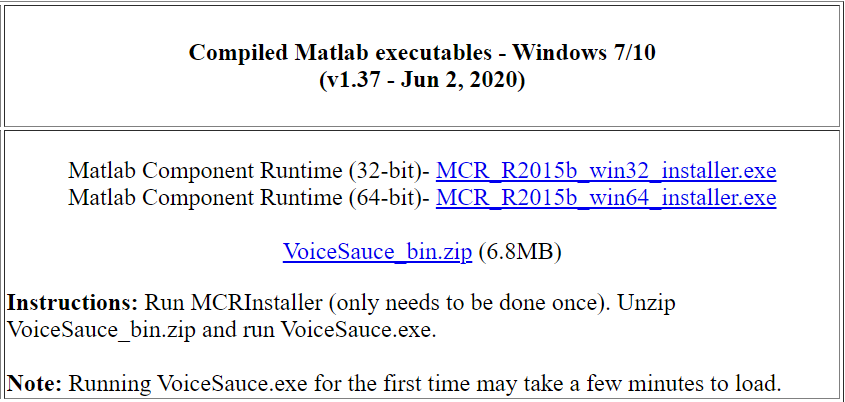
\includegraphics[width=0.5\textwidth,height=\textheight]{image/vs_windows_install_page.png}

  \begin{itemize}
  \tightlist
  \item
    To find out whether your computer has 32-bit or 64-bit system, go to
    ``Start'' → ``Settings'' → ``About''. On the main page you will see
    ``System type.''

    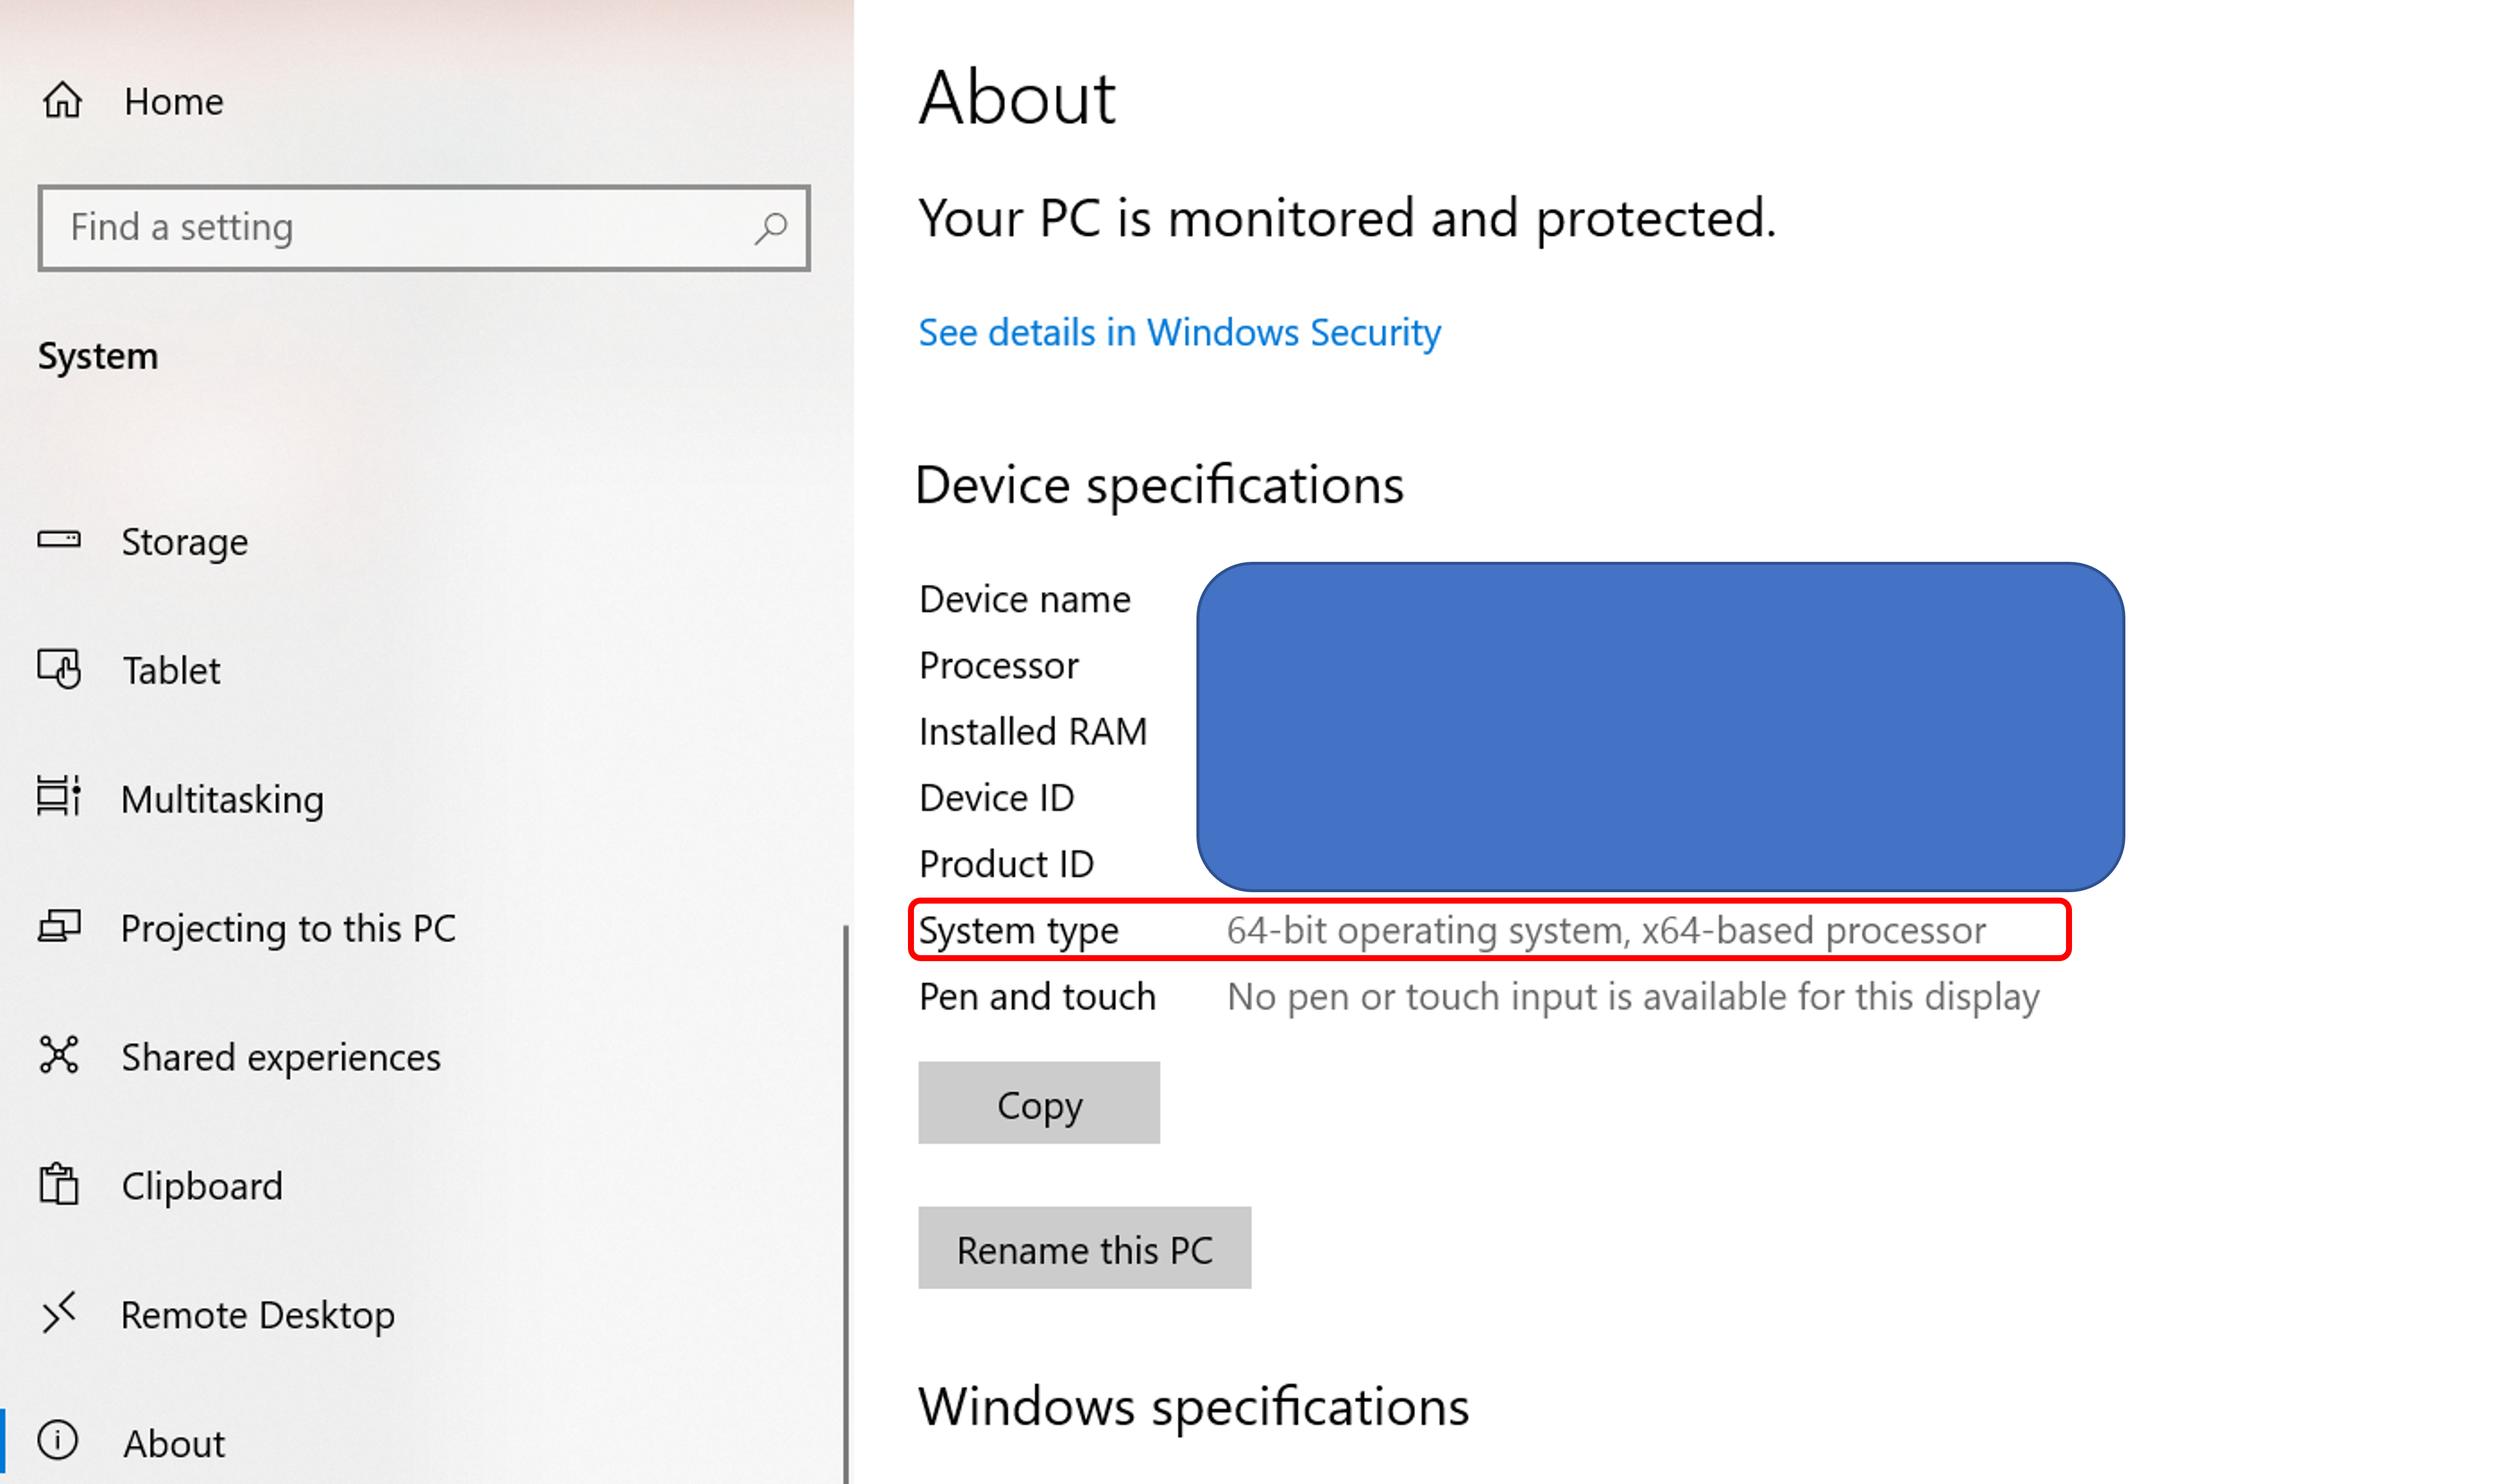
\includegraphics[width=0.5\textwidth,height=\textheight]{image/vs_system_type.png}
  \end{itemize}
\item
  Download VoiceSauce\_bin.zip, unzip the .zip folder, and click on
  VoiceSauce.exe to run the program.

  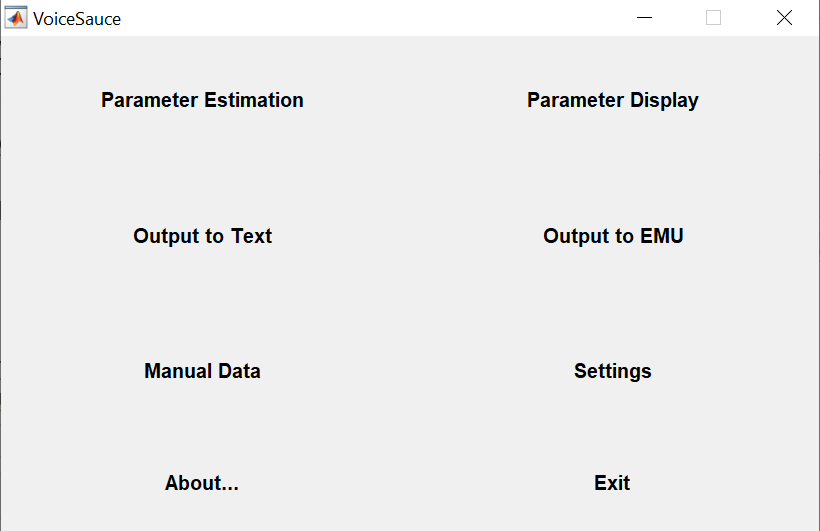
\includegraphics[width=0.4\textwidth,height=\textheight]{image/vs_windows_interface.png}
\end{enumerate}

\hypertarget{mac-users}{%
\subsection{Mac users}\label{mac-users}}

\begin{enumerate}
\def\labelenumi{\arabic{enumi}.}
\tightlist
\item
  Go to \url{http://www.phonetics.ucla.edu/voicesauce/}. Under ``Matlab
  m-code'', click on ``VoiceSauce.zip'' to download it. After download,
  unzip the VoiceSauce into a regular folder.

  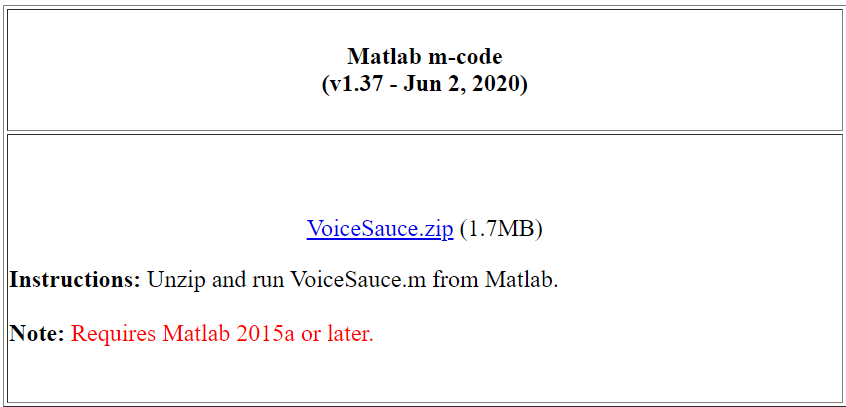
\includegraphics[width=0.5\textwidth,height=\textheight]{image/vs_matlabzip.png}
\item
  Install Matlab so that we can open VoiceSauce in Matlab:
\end{enumerate}

\begin{itemize}
\tightlist
\item
  Go to Matlab support at UHM:
  \href{https://www.mathworks.com/academia/tah-portal/university-of-hawaii-manoa-40591263.html}{here}.
  Click ``Sign in to get started''. Log in with your UH username and
  password.

  \begin{itemize}
  \tightlist
  \item
    New Users: Create a MathWorks Account. After entering your
    information, you will be sent an email to verify this account. Log
    in with your newly created MathWorks Account to download the
    software.
  \item
    Returning users: Log in with your MathWorks Account information to
    download the software.
  \end{itemize}
\item
  After logging into your Matlab account, select ``Install MATLAB''.
  Select ``R2022b'', click on ``Download for macOS''. Open
  ``matlab\_R2022b\_maci64.dmg''. The installation will start.
\item
  At the step of ``Select products'', select ``MATLAB'' and ``Signal
  Processing Toolbox''. Then proceed to the end of ``Begin install''.

  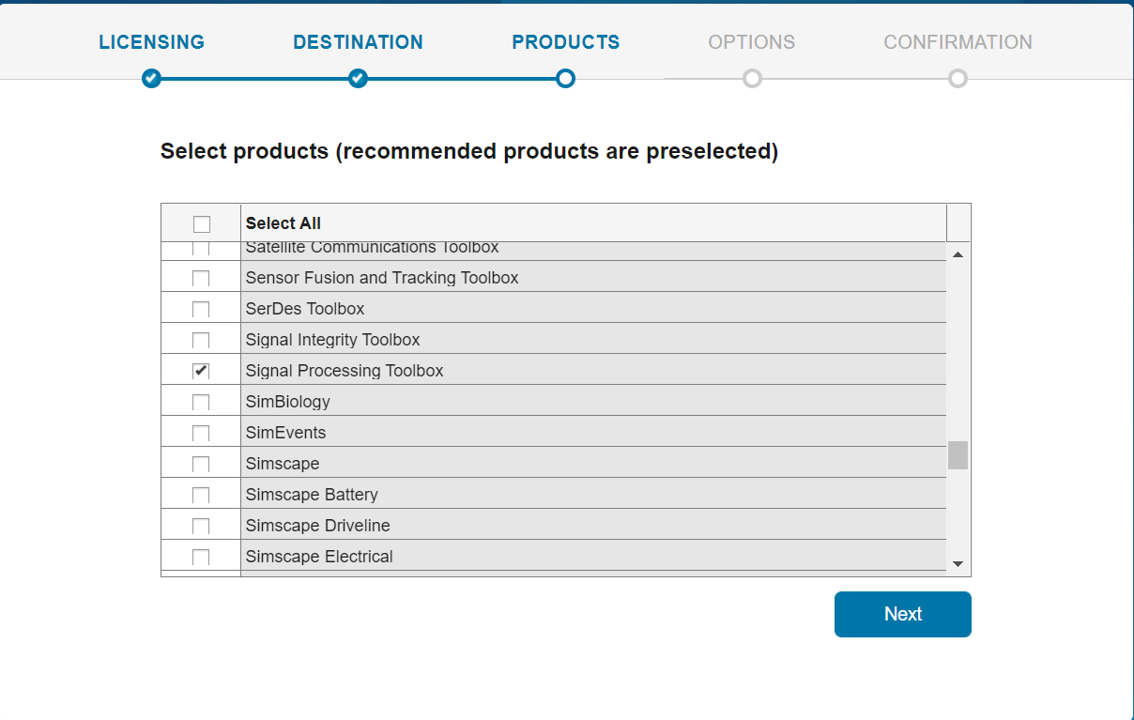
\includegraphics[width=0.5\textwidth,height=\textheight]{image/vs_mltoolbox.png}
\end{itemize}

\begin{enumerate}
\def\labelenumi{\arabic{enumi}.}
\setcounter{enumi}{2}
\tightlist
\item
  Open Matlab. Click on the rightmost icon at the address bar ``Browse
  for folder''. Navigate to the location where the VoiceSauce folder was
  stored. Select the VoiceSauce folder and click ``Select folder''.

  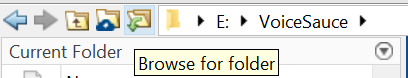
\includegraphics[width=0.3\textwidth,height=\textheight]{image/vs_ml_browsefolder.png}
\item
  On the left, find ``Current folder'' panel, find ``VoiceSauce.m'' and
  double left-click on the file.

  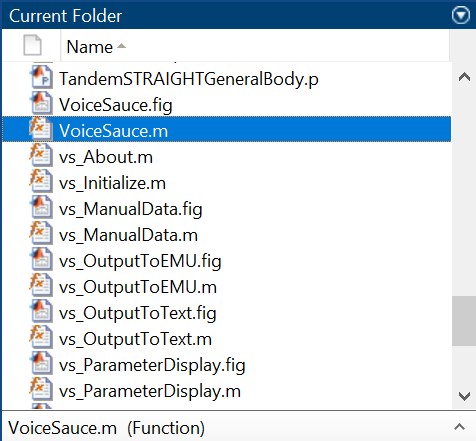
\includegraphics[width=0.3\textwidth,height=\textheight]{image/vs_ml_runvs.png}
\item
  The scripts show up in the Editor in the main panel. Under the tab of
  ``EDITOR'', click on ``Run''. The interface of VoiceSauce shows up.

  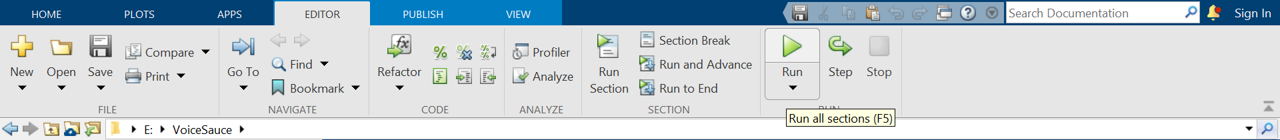
\includegraphics[width=0.7\textwidth,height=\textheight]{image/vs_run.png}

  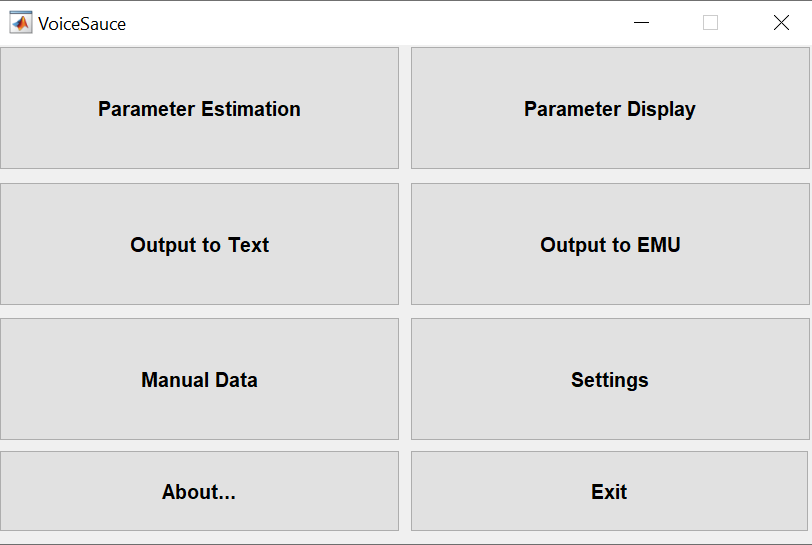
\includegraphics[width=0.4\textwidth,height=\textheight]{image/vs_ml_interface.png}
\end{enumerate}

\hypertarget{online-platform}{%
\subsection{Online platform}\label{online-platform}}

\begin{itemize}
\tightlist
\item
  Note that the online platform cannot compute formants or harmonic
  amplitudes with formant correction.
\end{itemize}

\begin{enumerate}
\def\labelenumi{\arabic{enumi}.}
\tightlist
\item
  Go to \url{http://www.phonetics.ucla.edu/voicesauce/}. Under ``Matlab
  m-code'', click on ``VoiceSauce.zip'' to download it.

  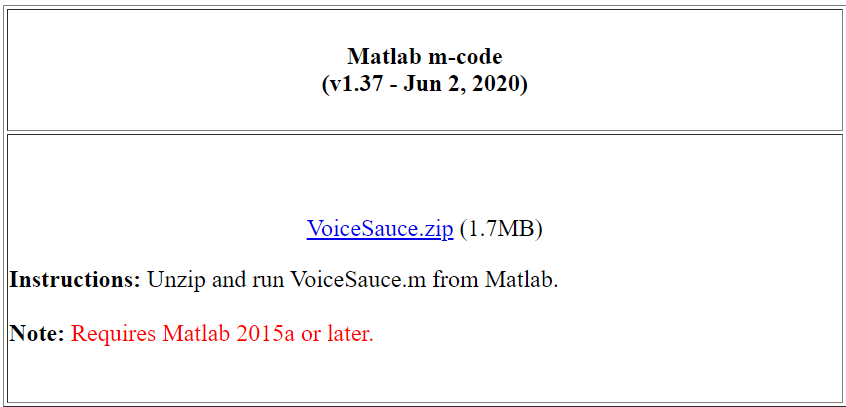
\includegraphics[width=0.5\textwidth,height=\textheight]{image/vs_matlabzip.png}
\item
  Go to Matlab support at UHM:
  \href{https://www.mathworks.com/academia/tah-portal/university-of-hawaii-manoa-40591263.html}{here}.
  Click ``Sign in to get started''. Log in with your UH username and
  password.

  \begin{itemize}
  \tightlist
  \item
    New Users: Create a MathWorks Account. After entering your
    information, you will be sent an email to verify this account. Log
    in with your newly created MathWorks Account to download the
    software.
  \item
    Returning users: Log in with your MathWorks Account information to
    download the software.
  \end{itemize}
\item
  After logging into your Matlab account, select ``Open MATLAB Online''.
  An online portal of Matlab opens.
\item
  Under ``Home'' tab, click on ``Upload'', navigate to the place where
  VoiceSauce.zip locates. Select VoiceSauce.zip.

  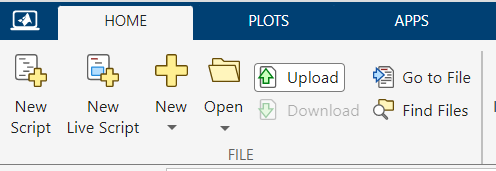
\includegraphics[width=0.4\textwidth,height=\textheight]{image/vs_import_online.png}
\item
  Under the left panel ``Current Folder'', double-click
  ``VoiceSauce.zip'' and unzip it. Click on the triangle besides the
  VoiceSauce folder to unfold it. Find ``VoiceSauce.m'' in the list and
  double click on it.

  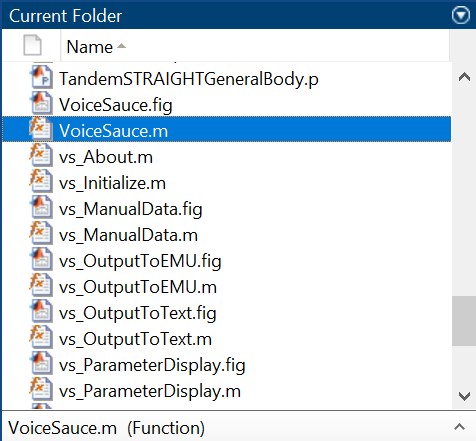
\includegraphics[width=0.3\textwidth,height=\textheight]{image/vs_ml_runvs.png}
\item
  Under the tab ``Editor'', click on ``Run''. If a prompt warns you that
  the script is not found in the path, select ``Add to path''. The
  interface of VoiceSauce shows up.

  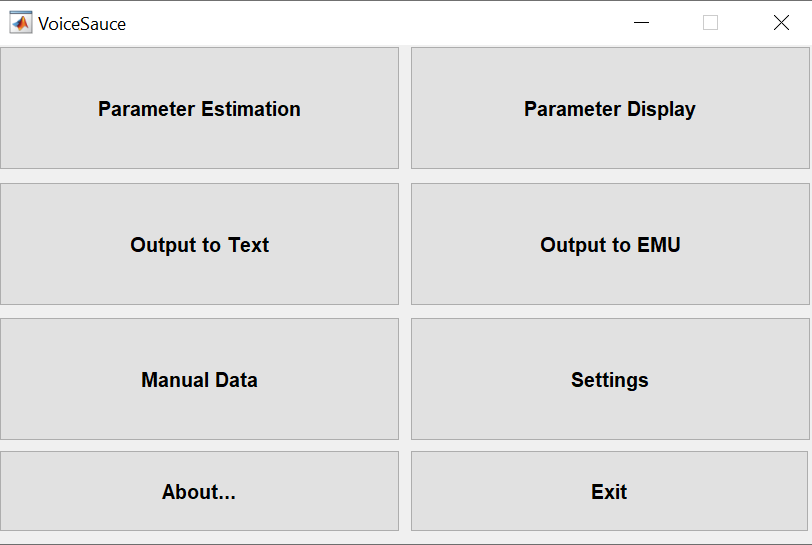
\includegraphics[width=0.4\textwidth,height=\textheight]{image/vs_ml_interface.png}
\end{enumerate}

\hypertarget{how-to-use-voicesauce}{%
\section{How to use VoiceSauce}\label{how-to-use-voicesauce}}

\hypertarget{prepare-your-.wav-and-.textgrid-files}{%
\subsection{Prepare your .wav and .Textgrid
files:}\label{prepare-your-.wav-and-.textgrid-files}}

\begin{itemize}
\tightlist
\item
  Put your audio file and TextGrid files in the same folder.

  \begin{itemize}
  \tightlist
  \item
    The .Textgrid file should have the same name as its corresponding
    .wav file. Avoid any special characters (e.g.~IPA symbols /ʔ, ə, ɯ/,
    letters with diacritics /ä, ã/).
  \item
    You can assign a different letter to the special characters and
    create a code sheet to keep a record of their correspondence.
  \item
    A sample folder with audio and Textgrid files can be found
    \href{sample/Indonesian_Stress_Soderberg_Olson_JIPA_2008.zip}{here}.
  \end{itemize}
\end{itemize}

\hypertarget{settings-in-voicesauce}{%
\subsection{Settings in VoiceSauce}\label{settings-in-voicesauce}}

\begin{itemize}
\tightlist
\item
  Click on ``Setting''. Under ``Common'', change ``Not a number label''
  as ``NaN''.

  \begin{itemize}
  \tightlist
  \item
    Other parameters that you can adjust:

    \begin{itemize}
    \tightlist
    \item
      F0: Max/Min F0
    \item
      Formants: Praat Max formant freq; Number of formants;
    \item
      Textgrid: Tier numbers (i.e.~if you have multiple tiers in your
      Textgrid file, which tier you'd like to analyze.)
    \end{itemize}
  \end{itemize}
\end{itemize}

\hypertarget{parameter-estimation}{%
\subsection{Parameter estimation}\label{parameter-estimation}}

\begin{enumerate}
\def\labelenumi{\arabic{enumi}.}
\tightlist
\item
  Click on ``Parameter Estimation''
\item
  Under ``Input (*.wav) directory'', click ``Browse'', navigate to the
  folder where your .wav and .Textgrid files are stored, and click
  ``select folder''. You will see a list of the files in that folder in
  the upper panel of the window.
\item
  If you'd like to save the output .mat files in the same folder with
  the sound, check ``Save *.mat files with *.wav files''. If you'd like
  a different location, navigate to that location under ``Output (*.mat)
  directory''.
\item
  Click ``Parameter Selection'' and select the parameters you want to
  estimate. If you do not have Praat installed, deselect F0 (Praat) and
  Formants (Praat).

  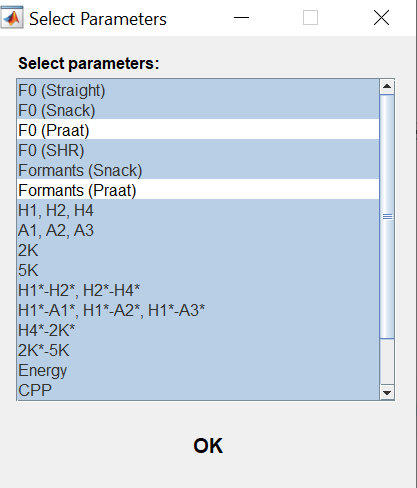
\includegraphics[width=0.4\textwidth,height=\textheight]{image/vs_parameter_selection.png}
\item
  Deselect ``Process using 16kHz sampling rate'' if that is not what you
  want. Check ``Use .Textgrid segmentation information if available''.
\item
  Click ``Start!'' to start the parameter estimation.

  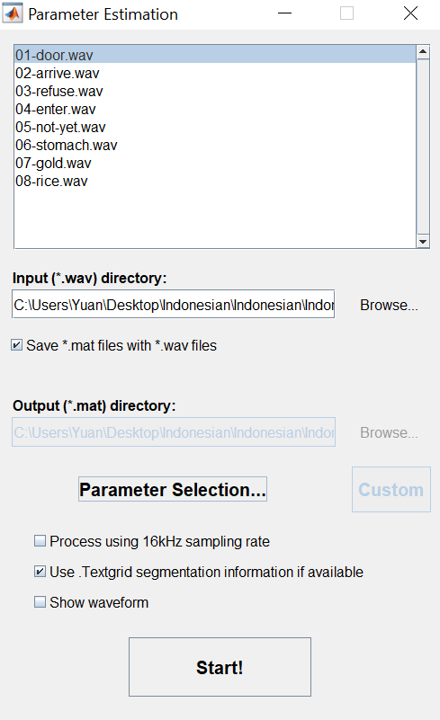
\includegraphics[width=0.4\textwidth,height=\textheight]{image/vs_parameter_estimation.png}
\item
  After seeing the message ``Processing complete'', close the window.

  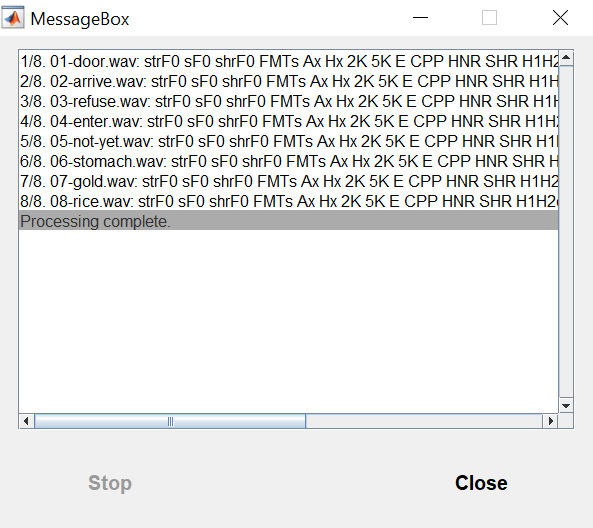
\includegraphics[width=0.4\textwidth,height=\textheight]{image/vs_processing_complete.png}
\end{enumerate}

\hypertarget{output-to-text}{%
\subsection{Output to Text}\label{output-to-text}}

\begin{enumerate}
\def\labelenumi{\arabic{enumi}.}
\tightlist
\item
  Click ``Output to Text''

  \begin{itemize}
  \tightlist
  \item
    Input .mat directory: where you saved the .mat output
  \item
    Input .Textgrid directory: where you saved the .Textgrid files
  \item
    Include EGG data: if you have EGG data that you want to include,
    navigate to the place where you saved .egg files
  \item
    Output .txt directory: where you want to save the .txt output
  \item
    Sub-segments:

    \begin{itemize}
    \tightlist
    \item
      No sub-segments: output all the data that are measured every 1
      millisecond
    \item
      Use sub-segments: the number of mean intervals you want to have
      for each target sound. E.g. if you enter ``3'', it will divide
      each target sound into three equal-timed intervals and calculate
      the mean value of each parameter for each interval.
    \end{itemize}
  \item
    Parameters: select the ones that you want to include in the .txt
    output
  \item
    Output Options:

    \begin{itemize}
    \tightlist
    \item
      Single file; You can customize the name of the output file under
      ``Output file''
    \end{itemize}
  \end{itemize}
\item
  An example output setting where I output H1*, H1*-H2*, CPP, Energy,
  HNR05, Formants, SoE and output only the mean for each target sound:

  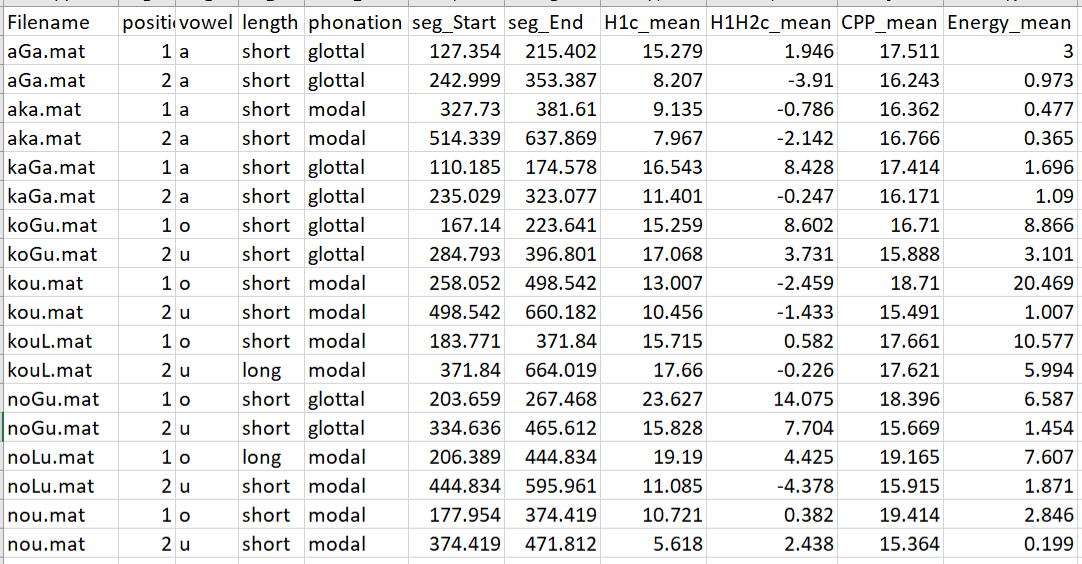
\includegraphics[width=1\textwidth,height=\textheight]{image/vs_outputtext.png}
\item
  After finishing the input, click on ``Start!''
\end{enumerate}

\hypertarget{analyze-the-output-in-excel}{%
\section{Analyze the output in
Excel}\label{analyze-the-output-in-excel}}

\hypertarget{open-the-output.txt-in-excel}{%
\subsection{Open the output.txt in
Excel}\label{open-the-output.txt-in-excel}}

\begin{itemize}
\tightlist
\item
  Go to ``Data'' tab → ``From Text/CSV'' → Navigate to the location
  where output.txt is saved and select ``output.txt''
\item
  Insert three empty columns after ``Label''
\item
  Split the ``Label'' by go to ``Data'' tab → ``Delimited'' → Other
  ``-'' → ``Next'' → ``Finish''
\item
  Change the column of ``Label'' as ``position''; Name the next three
  empty column heads as ``vowel'', ``length'', and ``phonation''.
\end{itemize}

\hypertarget{create-figures}{%
\subsection{Create figures}\label{create-figures}}

\begin{enumerate}
\def\labelenumi{\arabic{enumi}.}
\tightlist
\item
  Select the column of interest. For example, in the example data file
  for the acoustics of vowels surrounding glottal stop in Hawaiian, we
  will select the columns of ``phonation'' and ``HNR05\_mean''.

  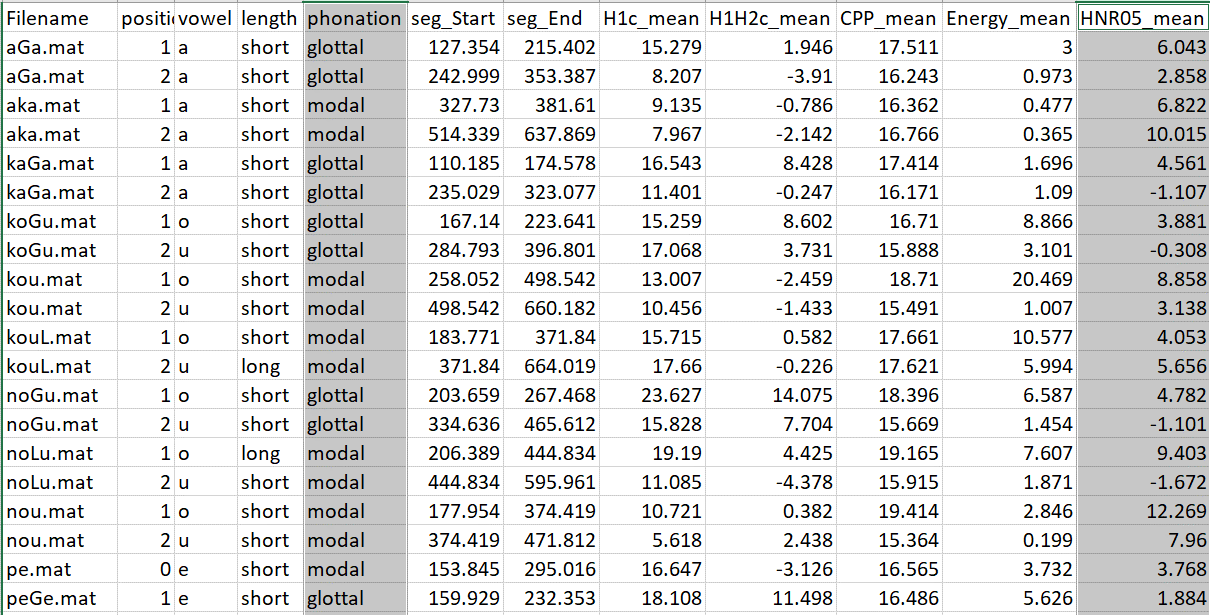
\includegraphics[width=1\textwidth,height=\textheight]{image/vs_selectcolumn_excel.png}
\item
  Go to tab ``Insert'' → ``Chart'' → ``Box \& Whisker'' → ``OK''. The
  figure is as below:

  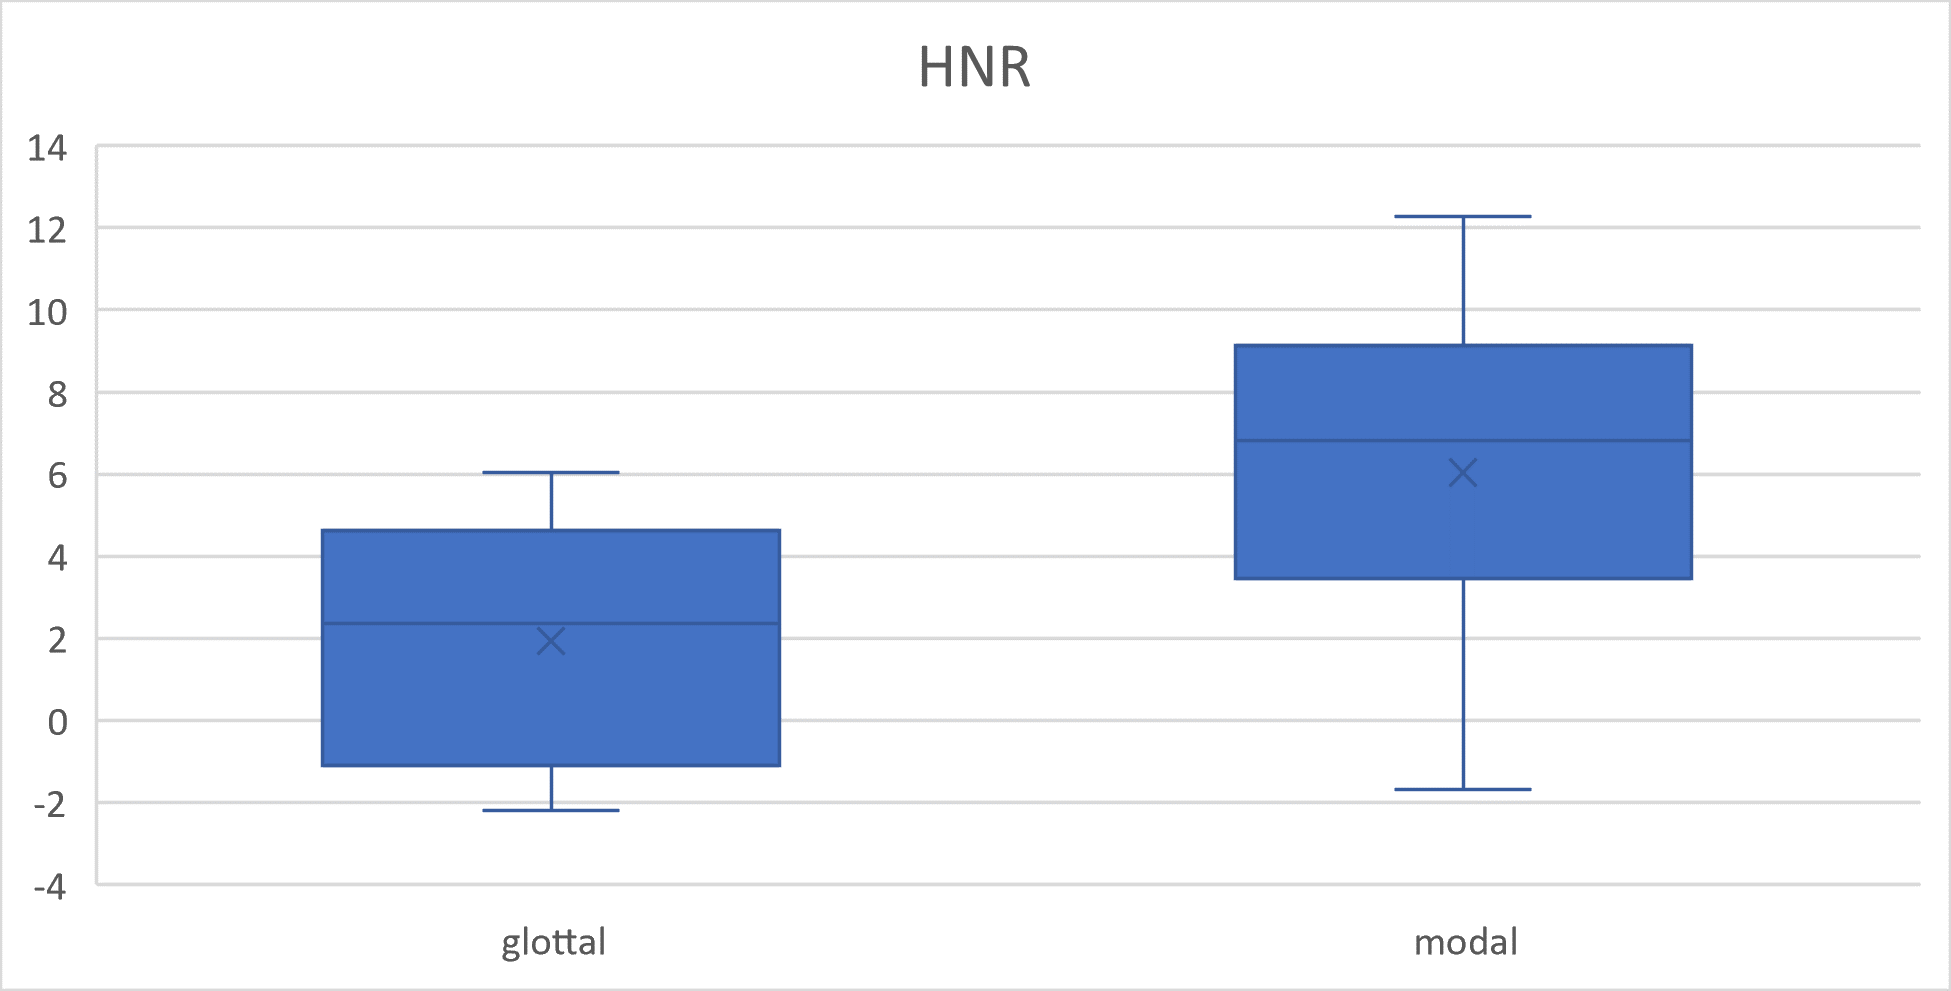
\includegraphics[width=0.7\textwidth,height=\textheight]{image/vs_samplehnrgraph.png}
\end{enumerate}

\end{document}
